\section{System} \label{sec:system}
\subsection{Signal model}

\begin{align}
  Y_{t}[n] &= S_{t}[n] + N_{t}[n] \quad \text{(time domain)}
  \label{eq:signal_time} \\
  Y_{k}[l] &= S_{k}[l] + N_{k}[l] \quad \text{(frequency domain)}
  \label{eq:signal_freq}
\end{align}

\begin{align}
  R_{S_{t}N_{t}}(n,m) &= 0 \quad \text{(uncorrelated)}
  \label{eq:signal_uncorrelated1} \\
  R_{Y_{t}Y_{t}}(n,m) &= R_{S_{t}S_{t}}(n,m) - R_{N_{t}N_{t}}(n,m)
  \label{eq:signal_uncorrelated2} \\
  R_{Y_{t}Y_{t}}(n,m) &= R_{Y_{t}Y_{t}}(m-n) \quad \text{(wide-sense stationary)}
  \label{eq:signal_wss}
\end{align}

\begin{align}
  P_{YY,k} &= \lim_{L \to \infty} \sum_{m=-L/2}^{L/2} R_{Y_{t}Y_{t}}(m) e^{-j2\pi \frac{km}{K}}
  \label{eq:pyyk1} \\
  &= P_{SS,k} + P_{NN,k}
  \label{eq:pyyk2} \\
  \hat P_{YY,k}^{P}(l) &= \frac{1}{L}\abs{Y_{k}(l)}^{2}
  \label{eq:pyyest} \\
  \hat P_{YY,k}^{B}(l) &= \frac{1}{M}\sum_{m=l-M+1}^{l} \hat P_{YY,k}^{P}(m)
  \label{eq:pyyBest}
\end{align}

\subsection{System overview}
\begin{figure}
  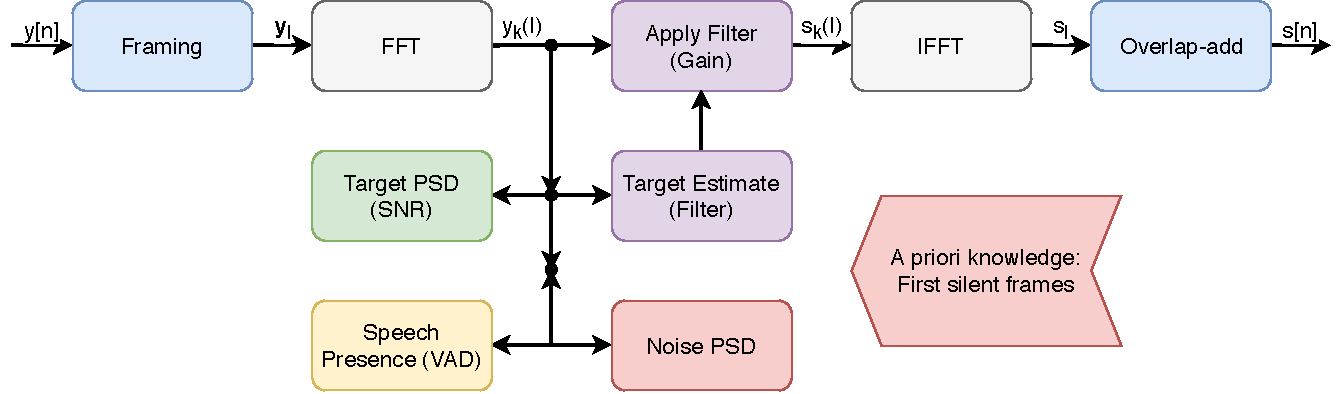
\includegraphics[width=\textwidth]{images/system.pdf}
  \caption{Overview of the system.}
  \label{fig:system}
\end{figure}
